\chapter{正文写作}
\label{c:main}
本章中介绍了一些\LaTeX 不得不说的基础知识,包括\LaTeX 语句的基本概念,\LaTeX 中的特殊字符,章节命令,空格、分行和段落等等。



\section{\LaTeX 语句}
\LaTeX 语句主要有命令、数据和注释组成。命令有控制词和控制符两种,其中控制词以右斜杠\verb|\|开始,以非字母字符结束(如\verb|\textbackslash|);控制符以\textbackslash 开始,紧跟着一个非字母、数字的字符(如\verb|\;|)。注释以\%开始,每行自\%之后的内容都不会被编译。

命令可能会有一些参数,如
\begin{code}
        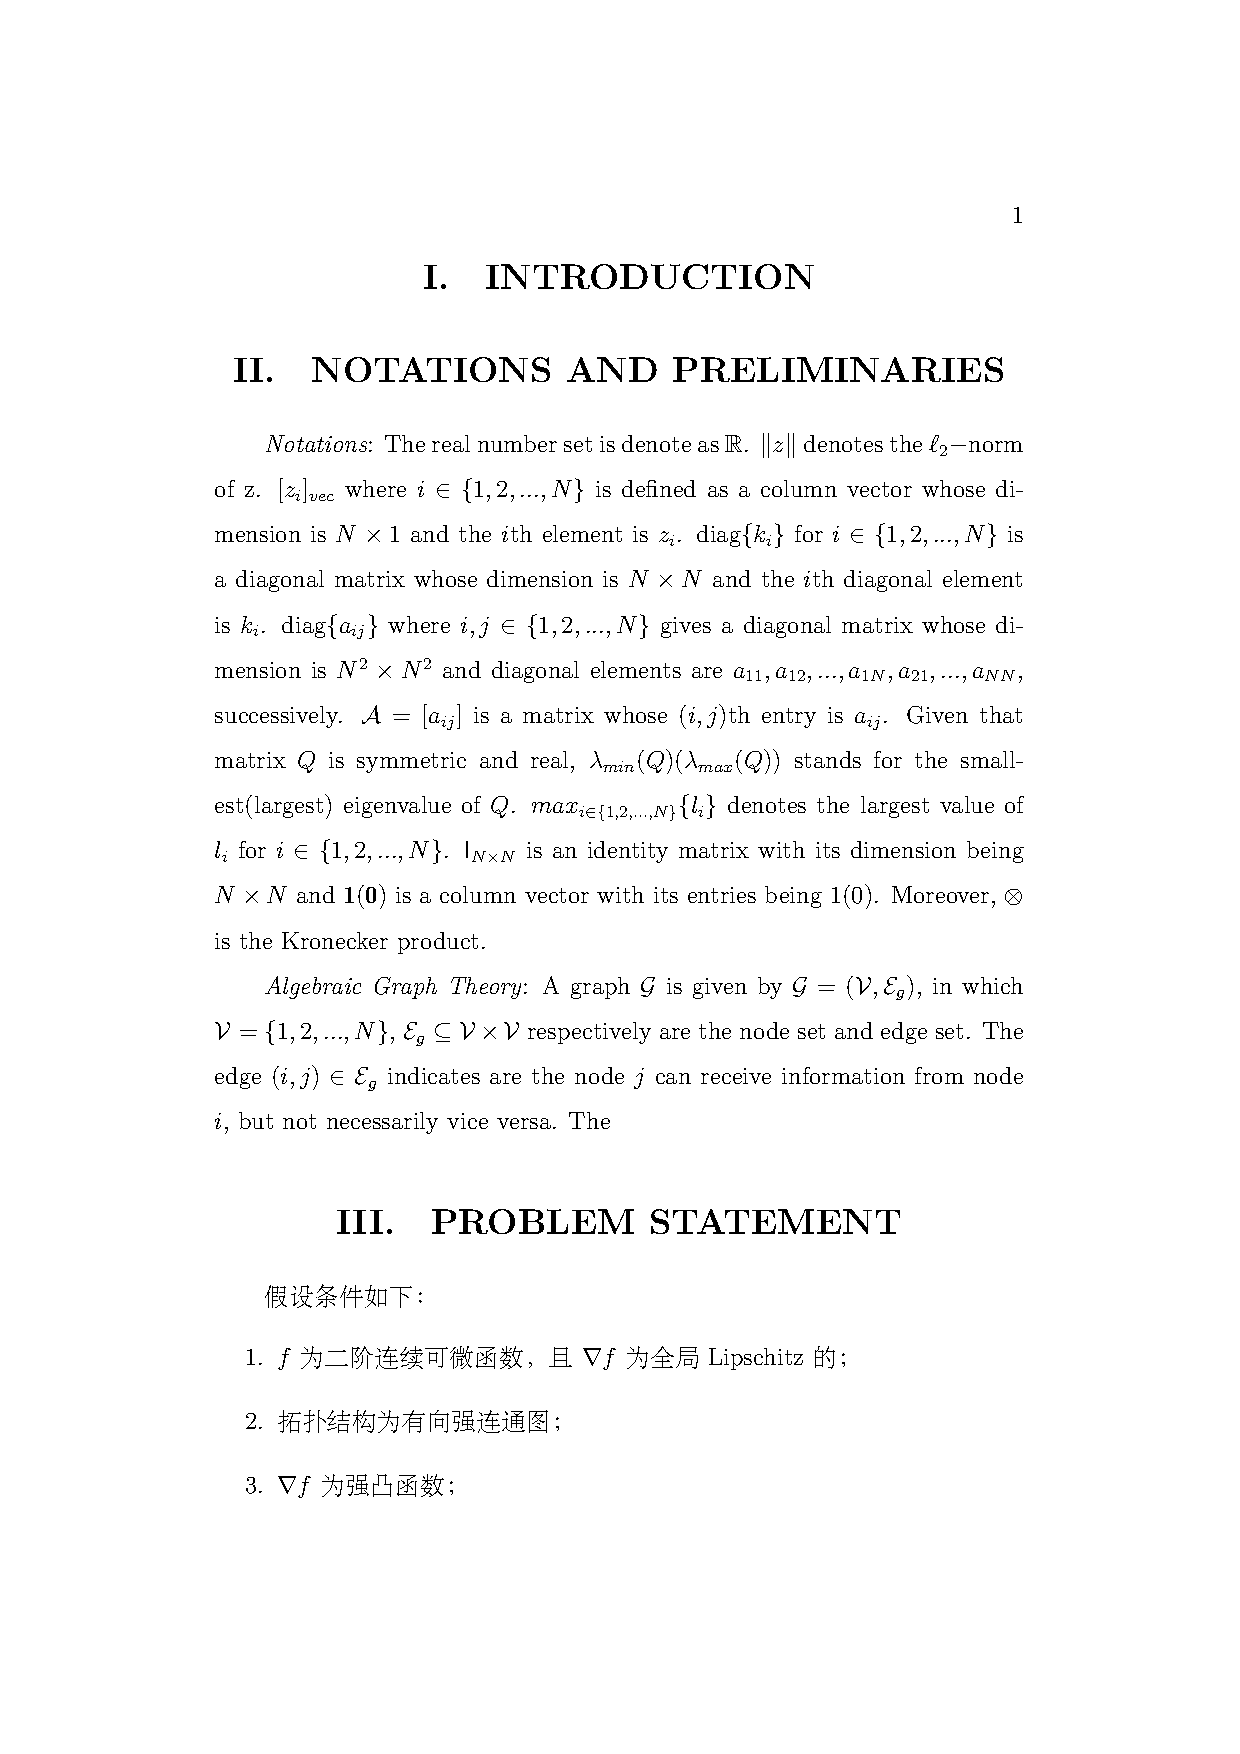
\includegraphics[width=10cm]{1.jpg}
\end{code}
其中中括号括起来的是可选参数,当省略时,\LaTeX{}会根据默认值来选择;大括号内的是不可省略的参数。这个命令的含义见第\ref{chap:fig}章。

\section{\LaTeX 中的特殊字符}
\subsection{空格与回车}
在\LaTeX 中,连续的空格被认为是一个空格。行首的空格通常被忽略。按下回车产生的断行也被认为是空格。\par
而当为了美观需要,不得不强行插入空格时,有很多选择,这里给出其中的一部分:
\begin{itemize}
\item{}\verb|~|,产生不可断行的半个空格;
\item{}\verb|\ |,即\verb|\|之后再加一个空格,产生1/3个字母m宽度空格;
\item{}\verb|\hspace{1cm}|,其中1cm可以随便替换,需要加长度单位,如em,pt等;
\item{}\verb|\quad|,一个字母m的宽度;
\item{}\verb|\qquad|,两个字母m的宽度;
\end{itemize}

一个回车会得到一个空格,而两个回车会得到一个空行,空行代表开始一个新段落。连续的空行被当作是一个空行。

\subsection{引号}
左右引号分别用不同的字符\verb|`|(数字1左边的键)和\verb|'|(通常所用的单引号)表示。双引号则是连续两个左引号+连续两个右引号。
\begin{figure}[h]
\centering
\fbox{\begin{minipage}[h]{0.4\textwidth}
我听见韩麦尔先生对我说:``唉,总要把学习拖到明天,这正是阿尔萨斯人最大的不幸。现在那些家伙就有理 由对我们说了:`怎么?你们还自己说是法国人呢,你们连自己的语言都不会说,不会写!……'不过,可怜的小弗郎 士,也并不是你一个人的过错。''
\end{minipage}}
\hspace{0.1\textwidth}
\begin{minipage}[h]{0.4\textwidth}
\centering
\begin{code}
我听见韩麦尔先生对我说:``唉,总要把学习拖到明天,这正是阿尔萨斯人最大的不幸。现在那些家伙就有理 由对我们说了:`怎么?你们还自己说是法国人呢,你们连自己的语言都不会说,不会写!……'不过,可怜的小弗郎 士,也并不是你一个人的过错。''
\end{code}
\end{minipage}
\caption{引号}
\label{f:quote}
\end{figure}

\subsection{控制字符}
以下这些是\LaTeX 中的控制字符:
\begin{code}
              #  $  %  ^  &  _  {  }  ~  \
\end{code}
它们被用作控制符,因而不能直接输入。要输入这些字符,分别可以用以下命令:
\begin{code}
        \#   \$  \%   \^{}  \&  \_  \{  \}  \~{}  \textbackslash
\end{code}
可以看到,一般来说,在这些字符前加上右斜杠\verb|\|,就可以正常输出。\verb|\\|除外,这是一个换行命令(见下一节)。\par

\subsection{横线}
一个短横线\verb|-|代表连字符,两个短横线\verb|--|会产生一个用于数字范围的短破折号,三个短横线\verb|---|产生普通的破折号。而代表负数的负号则应该是\verb|$-$|。

\section{控制字体样式}
大部分时候,\LaTeX{}会自动控制字样。当为了强调某些文字,需要改变字体时,以下有一些例子:
\begin{center}
\begin{tabular}{ll@\qquad ll}
\whline
\verb|\textrm{...}|& \textrm{roman}& \verb|\textbf{...}|& \textbf{bold face}\\
\verb|\textsf{...}| &\textsf{sans serif}& \verb|\textit{...} |&\textit{italic}\\
\verb|\texttt{...}|& \texttt{typewriter} &\verb|\textsl{...}|& \textsl{slanted}\\
\verb|\emph{...}|& \emph{emphasized}& \verb|\underline{...}|& \underline{underline}\\
\whline
\end{tabular}
\end{center}

表中列出了大部分常用的文字样式选择命令,使用时将需要改变字样的文字放在命令后的大括号中作为参数即可。

\section{改变字体大小}
ustcthesis模板中提供了字号选择命令:
\begin{code}
        \chuhao,\xiaochuhao,\yihao,\erhao,\xiaoerhao,...\qihao
\end{code}
一个简单的例子:
\begin{figure}[h]
\centering
\fbox{\begin{minipage}[h]{0.4\textwidth}
{\chuhao 初号}\\
{\sihao 四号文字}\\
{\qihao 七号文字}
\end{minipage}}
\hspace{0.1\textwidth}
\begin{minipage}[h]{0.4\textwidth}
\centering
\begin{code}
{\chuhao 初号}\\
{\sihao 四号文字}\\
{\qihao 七号文字}
\end{code}
\end{minipage}
\caption{字号选择}
\label{f:size}
\end{figure}

如例子中的那样,对于一段需要改变字号的文字,应当用大括号将其包围起来,将字号选择命令置于大括号开头。这样做可以防止字号选择命令影响之后的文字。

正文中默认使用的字号是小四号。

\section{控制空格,分行,分段,分页,章节}
\begin{description}
\item{\textbf{分行}}
这里我们说的是段内分行。在\LaTeX 中,普通的回车会被视为空格,而分行的命令则是\verb|\\|。分行与分段的区别在于下一行的段首不会缩进,并且
这两行之间的间距还是普通行间距,比段间距要小。
\item{\textbf{分段}}
一个空行意味着一段的结束和下一段的开始。也可以使用分段符:\verb|\par|。
\item{\textbf{分页}}
使用\verb|\newpage|命令强制分页。
\item{\textbf{章节}}
\LaTeX 使用章节类命令控制文章结构。章节类命令可以自动生成对应的格式,并且会自动插入目录中。\par
对于本科毕业论文,从大到小的章节依次为:\\
\begin{minipage}{0.8\textwidth}
\begin{code}
    \chapter,\section,\subsection,\subsubsection
\end{code}
\end{minipage}\\
章节命令的参数是该章节的名字。
\end{description}

\section{环境}
环境命令(environment)是一类特殊的\LaTeX{}命令。通常,一个环境命令定义了环境内部的字体、对齐和缩进方式、自动编号等信息,用于方便用户输入公式、注释、引文等。一个环境命令如下:
\begin{code}
            上文
            \begin{环境名}
                ...
                环境内的文字
                ...
            \end{环境名}
            下文
\end{code}

几个常用的环境有:
\begin{itemize}
\item center:居中
\item quote:引文
\item verbatim:原文照排,即不经过处理,直接按原样输出。
\item enumerate:自动编号的有序列表
\item itemize:枚举,带有项目符号的无序列表
\end{itemize}

\begin{example}{quote环境}\\
quote环境会自动设置缩进量和上下行距,如下图。
\begin{figure}[h]
\centering
\fbox{\begin{minipage}[h]{0.4\textwidth}
唐伯虎曾经写道:
\begin{quote}
别人笑我太疯癫,\\我笑他人看不穿。
\end{quote}
引自《桃花庵》。
\end{minipage}}
\hspace{0.1\textwidth}
\begin{minipage}[h]{0.4\textwidth}
\centering
\begin{code}
唐伯虎曾经写道:
\begin{quote}
别人笑我太疯癫,\\我笑他人看不穿。
\end{quote}
引自《桃花庵》。
\end{code}
\end{minipage}
\end{figure}
\end{example}

在itemize和enumerate环境中用item命令表示列举项。两者可以互相嵌套,如图\ref{f:item}。
\begin{figure}[!h]
\centering
\fbox{\begin{minipage}[h]{0.4\textwidth}
\begin{itemize}
\item fruit
\begin{itemize}
\item apple
\item strawberry
\end{itemize}
\item drinks
\begin{enumerate}
\item coffee
\item tea
\end{enumerate}
\item chocolate
\end{itemize}
\end{minipage}}
\hspace{0.1\textwidth}
\begin{minipage}[h]{0.4\textwidth}
\centering
\begin{code}
\begin{itemize}
    \item fruit
    \begin{itemize}
        \item apple
        \item strawberry
    \end{itemize}
    \item drinks
    \begin{enumerate}
        \item coffee
        \item tea
    \end{enumerate}
    \item chocolate
\end{itemize}
\end{code}
\end{minipage}
\caption{itemize和enumerate}
\label{f:item}
\end{figure}

关于其他数学环境以及公式的输入,请参阅第\ref{chap:math}章的相关内容。 